\documentclass[review]{elsarticle}

\usepackage{lineno,hyperref}
\usepackage[section]{placeins}
\usepackage{multirow}
\modulolinenumbers[5]

\journal{Journal of \LaTeX\ Templates}

%%%%%%%%%%%%%%%%%%%%%%%
%% Elsevier bibliography styles
%%%%%%%%%%%%%%%%%%%%%%%
%% To change the style, put a % in front of the second line of the current style and
%% remove the % from the second line of the style you would like to use.
%%%%%%%%%%%%%%%%%%%%%%%

%% Numbered
%\bibliographystyle{model1-num-names}

%% Numbered without titles
%\bibliographystyle{model1a-num-names}

%% Harvard
%\bibliographystyle{model2-names.bst}\biboptions{authoryear}

%% Vancouver numbered
%\usepackage{numcompress}\bibliographystyle{model3-num-names}

%% Vancouver name/year
%\usepackage{numcompress}\bibliographystyle{model4-names}\biboptions{authoryear}

%% APA style
%\bibliographystyle{model5-names}\biboptions{authoryear}

%% AMA style
%\usepackage{numcompress}\bibliographystyle{model6-num-names}

%% `Elsevier LaTeX' style
\bibliographystyle{elsarticle-num}
%%%%%%%%%%%%%%%%%%%%%%%

%define macros
\newcommand{\feature}[1]{{\ttfamily#1}}

\begin{document}

\begin{frontmatter}

\title{A Conceptual Framework for Evaluating and Designing Information Discovery and Curation Web Tools}


%% Group authors per affiliation:
\author[elenaemail]{Elena Voyloshnikova\corref{mycorrespondingauthor}}
\author[peggyemail]{Margaret-Anne Storey}

\address{University of Victoria}
\address{3800 Finnerty Rd, Victoria, BC, Canada, V8P 5C2}

\address[elenaemail]{elenavoy@uvic.ca}
\address[peggyemail]{mstorey@uvic.ca}

%% or include affiliations in footnotes:
\cortext[mycorrespondingauthor]{Corresponding author}
\ead{elenavoy@uvic.ca}




\begin{abstract}
Everyday life involves the discovery and curation of digital information. People search the Web continuously, from quickly looking up information needed to complete a task, to endlessly searching for inspiration and knowledge. A variety of studies have modeled information seeking strategies and characterized curation activities on the Web. However, there is a lack of research on how existing Web applications support the discovery and curation of information, especially concerning user motivations and how different approaches can be compared. This paper presents a study of information discovery tools and how they relate to the nature of information seeking. We propose a conceptual framework of application design elements that support different aspects of information discovery and curation. This framework can be used for designing, evaluating and updating Web applications.
\end{abstract}

\begin{keyword}
Information discovery \sep information curation \sep Web design
\end{keyword}

\end{frontmatter}

\linenumbers

\section{Introduction}

Web technologies help people satisfy their information needs. People research their interests and hobbies using various online resources, shoppers search online stores for product characteristics to make purchasing decisions, and travelers visit online booking sites to find information about flights and hotels. To accommodate diverse and evolving user needs, Web applications continuously introduce new features and services, empowering information discovery and curation. 

The term ``information discovery'' has been used to define or explain various information behaviour paradigms, such as information exploration~\cite{waterworth1991model} and serendipitous information seeking~\cite{foster2003serendipity}.  
Information discovery can take on many forms. Web users might be hoping to find particular pieces of information, such as show times and phone numbers, to satisfy specific information needs~\cite{proper1999information}. Alternatively, they might be lacking well-articulated information needs, so they engage in opportunistic browsing~\cite{lindley2012s}. Sometimes people discover information online without even looking for it~\cite{bates1986exploratory}. The nature of information discovery can vary, and therefore, requires elaborate tool support. With people having such diverse information needs and methods of looking for information, designing for information discovery is a challenging task~\cite{conaway2010designing, marchionini2006exploratory}.

Our research goal is to gain an understanding of how existing tools support digital information discovery and curation so that we can improve the design of Web applications for information discovery. While several researchers propose frameworks targeted at designing information discovery systems~\cite{proper1999information, kerne2004information}, the importance of information curation in the realm of information discovery has been largely overlooked despite the rapidly increasing popularity of socially-curated information spaces. Moreover, much of the existing work that focuses on how people look for and discover information online~\cite{bates1986exploratory, choo2000information, ellis1989behavioural, kellar2006goal, lindley2012s, morrison2001taxonomic, sellen2002knowledge} fails to examine concrete features of existing Web-based information discovery applications that empower real-world users. More research is necessary to determine how different tool features provide fundamental support for information discovery and curation.

To enhance information seeking and curating experiences and support users' interactions, we extend existing research by: (1) deriving factors that enable information discovery and curation and relating them within a framework; (2) using the framework to establish a set of questions for evaluating and designing new applications; (3) iteratively evaluating the framework by using it to study and describe current Web applications, which in turn helped refine the framework of factors and questions; and (4) relating the framework to information discovery and curation motives that drive the underlying usage of Web-based applications.

\section{Web-based Information Discovery and Curation}
\label{section:literature_review}
Given the complexity of Web-based information discovery and curation tasks, a variety of research topics are examined to gain an understanding of how current Web tools support these tasks, including information-related Web usage characteristics and current information behavior models.

% CUTCANDIDATE
%, and other aspects of information discovery and curation.  
%This section outlines key literature that contributes to the development of our conceptual framework.
% CUTCANDIDATE

\subsection{Information Behavior}
Information behavior refers to the totality of ways in which humans behave in relation to information~\cite{wilson2000human}.  A number of models and frameworks have attempted to represent human information behaviour in its entirety or to represent some of its components, such as information seeking and searching, information discovery, and information curation. 

% CUTCANDIDATE
%One of the early information behavior models was proposed by Wilson~\cite{wilson1981user} in 1981. It states that information seeking behavior results from the user trying to satisfy a perceived information need, and consequently, the user makes demands on information systems. Success or failure of such demands dictates whether the process is repeated or, if the information need is satisfied, is used or communicated with other people. These underlying ideas remained in the revision of Wilson's model~\cite{wilson1997information} in 1997. In the new model, however, Wilson defined possible barriers (psychological, environments, demographic, etc.) that can impede information seeking. Additionally, the model recognizes that information seeking behaviour can take on many forms and is not limited to active searching. 
% CUTCANDIDATE

\subsubsection{Information Seeking Models}
\textit{Information seeking} refers to ``the purposive seeking for information as a consequence of a need to satisfy some goal~\cite{wilson2000human}.'' Several researchers have tried to identify what different modes of information seeking behaviour may entail. According to Kellar et al.~\cite{kellar2006goal}, information seeking is composed of browsing, fact finding, and information gathering. Although the authors categorized information gathering as part of information seeking, it appears to be more closely related to digital curation~\cite{beagrie2008digital,whittaker2011personal}. 
%Bates~\cite{bates1986exploratory,bates2002toward} proposed a model of four information seeking modes: being aware, monitoring, browsing, and searching. Bates differentiated the modes based on the user's level of attention being active or passive, and their information needs being directed or undirected. 
Ellis et al.~\cite{ellis1989behavioural,ellis1993comparison,ellis1997modelling} proposed a model of information seeking characterized by six different patterns: starting, chaining, browsing, extracting, monitoring, and differentiating. 
% CUTCANDIDATE
%Ellis' model complemented Kuhlthau's work, which correlated stages of information seeking with feelings, thoughts, actions, as well as anticipated information tasks~\cite{kuhlthau1991inside}.
% CUTCANDIDATE

\subsubsection{Information Foraging}
\textit{Information foraging theory} is another approach towards understanding how people adapt their strategies of interacting with technology when seeking, gathering, or consuming information, depending on the environment~\cite{pirolli1999information}. The theory resonates with explanations of human behavior in the context of food foraging. The underlying assumption of the information foraging theory is that people, similarly to when they forage for food, adopt their foraging strategies to the environment in order to gain the maximum amount of valuable information. The theory states that ``natural information systems evolve towards stable states that maximize gains of valuable information per unit cost.''
%
The theory introduces three key concepts to formulate an understanding of information foraging: 
1) \textit{information scent} that refers to proximal cues (often visual or linguistic) that people use to identify the value of information; 2) \textit{information diet} which deals with user preferences when it comes to information and 3) \textit{information patches} that are clusters of information that an information system presents before the user. This theory lays the foundation for existing information foraging models~\cite{fu2007snif,kitajima2000comprehension} as well as social information foraging models~\cite{pirolli2009elementary,fu2008microstructures}.  


\subsubsection{Information Discovery}
Kerne and Smith proposed an information discovery framework~\cite{kerne2004information} that connects human cognitive states 
to those of an information system. The framework represents a continuum of information flowing through different system and cognitive states as a result of an iterative reformulation process. The framework consists of five mental states: formulating a problem, evaluating results, updating and forming mental models, running mental models, and discovering solutions. Each mental state has a corresponding interaction with the system. For example, browsing resources (human-system interaction) facilitates evaluation of immediate results (cognitive state). 
% CUTCANDIDATE
%The framework helps to understand the user's cognitive processes and provide affordances that facilitate information discovery.
% CUTCANDIDATE
   
\subsubsection{Digital Curation}
In 2002, Bates extended her research on the topic of information behaviour with the notion of \textit{information farming}, which involves people collecting and organizing information for future use and revisitation~\cite{bates2002toward}. More commonly, information farming is referred to as digital curation. Whittaker suggests that in terms of Web use, a significant shift is happening from information consumption to information curation. People no longer use the Web just to find and consume information of interest, but they also try to save and manage that information to refind and exploit later~\cite{whittaker2011personal}. 

In summary, existing models and frameworks for information seeking, searching, exploration, discovery and curation try to explain human information-related behavior using different but comparable terminology. They help establish an understanding of how humans interact with information, however, they fail to address the required tool support for information-related activities or they address the needs at too high a level.  

\subsection{Web Tasks and Modes of Web Use}
Outside the realm of cognitive models and frameworks for information behavior, we find research that examines information discovery, curation, and other Web information behaviours and corresponding tasks, methods, and modes.

Kellar et al.~\cite{kellar2006goal} separated Web tasks into five categories: transactions, browsing, fact finding, information gathering, and other uncategorized tasks. In later work, Kellar et al.~\cite{kellar2007field} added communication and maintenance as additional Web tasks. Similarly, Sellen et al.~\cite{sellen2002knowledge} identified six tasks that are performed by Web users: browsing, finding, housekeeping, information gathering, communicating, and transacting. Using different terms, Kellar et al. and Sellen et al. both identified highly comparable tasks, such as fact finding and finding [information], housekeeping and maintenance, etc. 

Building on Ellis' model of information seeking~\cite{ellis1989behavioural,ellis1993comparison,ellis1997modelling}, Choo et al.~\cite{choo2000information} derived anticipated Web tasks that correspond to the information seeking patterns in the model, such as identifying which Websites would point to information of interest, navigating through links, bookmarking, etc.  
%According to the authors, when users \textit{identify} sources of interest, they usually identify which Websites can point to that information of interest.  \textit{Chaining} occurs when users navigate through links on those initial pages. When people \textit{browse}, they scan top-level pages, headings, lists, and site maps. \textit{Differentiating} takes place when people bookmark, print, copy and paste information, or choose an earlier selected site. \textit{Monitoring} occurs when users revisit or receive updates from previously visited sites. Finally, \textit{extraction} occurs when the user systematically searches sites to extract information of interest.  

People often engage in information seeking activities to close some knowledge gap that occurred as a result of not having enough information to perform a task~\cite{proper1999information}. Therefore, when providing tool support for various information discovery tasks, it is useful to consider the motivations as they can be different for each task. Morrison et al.~\cite{morrison2001taxonomic} make a distinction between methods of Web use and purposes. The authors derived a purpose-based taxonomy of Web use, including three purposes or motivations: finding information, comparing pieces of information or choosing products to make a decision, and using the Web to find relevant information to gain an understanding of some subject. Consequently, methods of finding information identified by Morrison et al. are collecting, finding, exploring, and monitoring. The differences between the two taxonomies suggest that different information seeking tasks may be performed to satisfy more than one information seeking purpose. Therefore, each purpose may require more than one task-supporting mechanism. 
%Morrison et al. also draw a distinction between finding or looking up information and exploratory search. Whereas information lookup involves tasks such as fact retrieval, navigation, and verification, exploration is more cognitively demanding and involves learning and investigation~\cite{marchionini2006exploratory}. 
%Learning and investigation can be performed over multiple iterations and can involve learning though various media,``social searching", and serendipitous browsing to support knowledge acquisition, socialization, forecasting, and planning.  

Categorizing Web usage into information seeking, digital curation, and other Web tasks may not adequately describe how information-related tasks are performed. Lindley et al.~\cite{lindley2012s} conducted a qualitative study and
% CUTCANDIDATE
%involving 24 participants, tracking their daily Web usage in the form of a diary. They 
% CUTCANDIDATE
identified five distinct modes of Web use: respite, orienting, opportunistic, purposeful, and lean-back. 
% CUTCANDIDATE
%Lindley et al.'s primary motivations behind looking at use modes that occur when people browse the Internet were because traditional Web use studies and Web tasks discovered by other researchers have not reflected the depth of users' online intentions. 
% CUTCANDIDATE
Understanding the characteristics of different modes can guide the design of Web interactions. For example, opportunistic use can have unarticulated or continuously changing information needs. 
%People often cannot indicate the completion of Web tasks and finish whenever they have been browsing the Internet for too long or whenever they need to complete a higher priority task. 
Later they may resume their opportunistic information seeking.  Opportunistic use is also `grasshopper-like' as users often jump from one resource to another~\cite{lindley2012s}.
% CUTCANDIDATE 
%From these factors, we can assume that to support such Web usage, 
%we would 
% CUTCANDIDATE
Thus, there is a need to consider mechanisms for supporting users' information needs, revisitation, and arbitrary navigation.

Different taxonomies of information seeking and curation tasks reflect on actual Web usage rather than theoretical modeling of human behavior, however, these taxonomies still focus on human activities when they interact with technology. A better understanding of how a system can support these activities is needed in order to effectively support human information-related interactions. 

%\subsection{Summary}
In summary, there are a multitude of tools that support different aspects of information discovery and curation, but understanding how these tools are similar (or differ) is difficult. Moreover, the existing research is not useful for identifying gaps in current tools or ways that current tools may be improved to support information discovery and curation. We address these problems by presenting a conceptual framework for information discovery and curation.

\section{Methodology}
\label{section:methodology}
Our methodology consisted of four steps. To gain a deeper understanding of the problem of information discovery and curation, we conducted an extensive literature review where we derived a preliminary set of information discovery and curation design factors and related them within a framework. The framework was then applied as part of the evaluation of 20 different information discovery applications and iteratively refined after every evaluation. Lastly, the framework was applied to a reevaluation of some of the previously evaluated tools with the purpose of validating its effectiveness. 

{\subsection{Research Questions and Objective}
This study was designed to address the problem of designing Web applications for information discovery and was motivated by the following:

\emph{RQ1:~How do existing Web applications support information discovery?}

\emph{RQ2:~How do existing information discovery applications support information curation?}

To address RQ1 and RQ2, we conducted an extensive literature review and a case study of 20 information discovery tools. Using insights from RQ1 and RQ2, we established our main research objective: \emph{\textbf{to develop a framework for performing summative and formative evaluation of Web-based information discovery and curation tools}}.

}% end section

{\subsection{Literature Review}
\label{subsection:lit_review}
The development of the framework began with an extensive literature review. A diverse set of topics contributed to forming an understanding of information discovery and curation, including information behaviour and information seeking models, high-level Web tasks, and modes of Web use, exploration-based models of discovery, and methods of personal and social curation. From this review, the preliminary design factors for the framework were derived.
}% end section

{\subsection{Building and Refining the Conceptual Framework}
\label{subsection:building}
The Conceptual Framework we present in this paper was iteratively developed and refined through a careful analysis of 20 information discovery applications (see Table~\ref{table:tools}) and an in depth literature review.   
% CUTCANDIDATE 
%, the framework was iteratively expanded by adding new concepts and establishing relations between those concepts.  
%The framework was refined as we explored the literature and available tools---for presentation purposes, this paper covers two versions of the framework. The final version of the framework was a result of developing an information discovery application based on the preliminary work. 
% CUTCANDIDATE    
%
To guide the development of the framework, we selected some of the most used information discovery applications today.
% CUTCANDIDATE
% and considered the full range of features in those tools (both by referring to the literature and documentation on those tools, as well as exploring the features). 
 % CUTCANDIDATE
The popularity of information discovery applications was determined using Website popularity ranks provided by Alexa\footnote[1]{Alexa is available at www.alexa.com}, a commercial Web traffic data provider. The focus was on applications that had strong information discovery components and less priority was given to applications whose purpose revolved only around curation.
%
% CUTCANDIDATE
%We used Yin's case study design strategies~\cite{yin2014case} for guidance. The motivation behind choosing a case study over other methods of qualitative research was based on our choice of research questions, the lack of control over existing applications and their development, and having to focus on contemporary use of real-life Web applications. According to Yin~\cite{yin2014case}, a case study would be an optimal research strategy given the above characteristics.
%Our study consisted of 20 cases, with each case involving a Web application focused on the support of information discovery. 
% CUTCANDIDATE
We examined the overall purpose of each application, its description as defined within the application, as well as literature and documentation related to the application (if they were available) against the features that the application provided. For example, if an application provided bookmarking features, we checked if it was indeed intended to be used for information preservation. 

Our methodology involved an iterative process of selecting tools, analyzing them, and determining whether they could be described and evaluated using the framework. If we found a key feature that could not be described, we adapted the framework according to the findings. We repeated the process of tool selection and evaluation until the framework was usable for all tools. We then grouped the elements of the framework into categories, recording corresponding questions to ask in order to evaluate other applications. 
%
%A list of the tools that were used in this study are presented in Table~\ref{table:tools}.
% CUTCANDIDATE
% Other tools were considered throughout the study, however, only the 20 applications listed underwent systematic examination. 
 % CUTCANDIDATE

\begin{table}[htbp]
\small
\begin{tabular}{|p{0.23\columnwidth}| p{0.32\columnwidth}| p{0.32\columnwidth}|}

\hline
\textbf{Application} & \textbf{Address} & \textbf{Description}
\\
\hline
Pinterest       & www.pinterest.com 	& Visual discovery tool \\
\hline
Delicious       & delicious.com 		& Social bookmarking service \\
\hline
Tumblr          & www.tumblr.com 		& Microblogging platform \\
\hline
StumbleUpon     & www.stumbleupon.com  	& Web page discovery tool \\
\hline
Wikipedia       & en.wikipedia.org   	& Free content Internet encyclopedia\\
\hline
Google Maps     & www.google.ca/maps  	& Web mapping service\\
\hline
Rotten Tomatoes & www.rottentomatoes.com & Movie and TV database\\
\hline
500px           & 500px.com            	& Photography site\\
\hline
BucketList      & bucketlist.org  		& Goal tracking and discovery service\\
\hline
We Heart It     & weheartit.com 		& Visual discovery tool \\
\hline
Scoop.it!       & www.scoop.it 			& Online publishing platform \\
\hline
Google Images   & images.google.com  	& Image discovery service \\
\hline
Vimeo           & vimeo.com  			& Video sharing Website\\
\hline
LifeHacker      & lifehacker.com        & Daily blog \\
\hline
YouTube         & www.youtube.com 		& Video hosting platform \\
\hline
Yelp            & www.yelp.ca  			& Business review site\\
\hline
IMDb            & www.imdb.com  		& Movie database \\
\hline
Trip Adviser    & www.tripadvisor.ca 	& Travel site \\
\hline
Urban Spoon     & www.urbanspoon.com    & Online bar and restaurant guide\\
\hline
Thesaurus       & thesaurus.com         & Online thesaurus \\
\hline
\end{tabular}
\caption{Web-based Information Discovery and Curation Tools Studied}
% as of May 15, 2014}
\label{table:tools} 
\end{table}
} % end section

{\subsection{Framework Validation}
\label{subsection:validating}
% ELENA: check this!
In order to demonstrate the benefits of having such a framework, we applied the framework to five of the previously examined tools and show how its application can help in describing (and comparing) the features of these tools while revealing how the tools may be improved. Furthermore, we used the framework to guide the design of a novel tool.  Due to space constraints, we can only report one of these results here (see Section Framework Validation) and we direct the reader to~\cite{voyloshnikova2015} for full details on this validation.    

{\subsection{Limitations}
The case study we conducted has a number of limitations. A lack of documentation, research literature, and formal descriptions of available features for some applications introduces a threat to the construct validity of the study. In addition, information discovery tools and features can be used in unintended or unforeseen ways by designers and developers. Therefore, the recorded use of some features within information discovery applications was recorded in our interpretations. To compensate for such limitations, the researchers personally employed the tools over an extended period of time to gain a deeper understanding of their use. In addition, we considered some cases with similar functionality and design to be able to validate or clarify prior findings. 
% CUTCANDIDATE
%Many Web applications evolve rapidly. Therefore, our tool analysis only applies to tools at the moment of the study. 
% CUTCANDIDATE
Additionally, framework validation was performed on five of the previously examined tools, introducing another limitation. 
%
%Only Web applications running in browsers on a desktop computer were considered in this study. The study can be extended to various devices, such as smartphones and tablets, as information discovery patterns and mechanisms may vary for different platforms. 
% CUTCANDIDATE

Another limitation was the lack of prior research on the subject matter. Some researchers have studied information seeking models and high-level Web tasks, but there is a lack of literature on how to enable and support different Web tasks. This opens up opportunities for future research to analyze methods of developing and building frameworks for facilitating and evaluating tools that support other Web tasks, such as communication, transactions, and goal realization.
}
\section{A Conceptual Framework for Information Discovery and Curation on the Web}
\label{sec:framework}

In our framework, we build on existing models and frameworks of information discovery and curation and our analysis of existing Web tools to derive corresponding design factors for Web design. The first part of the framework deals with the \textit{motives} behind information discovery and curation. These motives often define use cases for Web application design and help set initial assumptions about the required functionality.

The second part of the framework defines the \textit{actions} that comprise discovery and curation activities, and the design factors that enable them. Some examples of actions include managing and preserving information. To support these actions, a Web-based application must provide corresponding mechanisms, such as bookmarking and tagging capabilities.

Actions can be further decomposed into \textit{operations} performed using mechanisms that enable the actions. For example, the information preservation (action) can be enabled using a bookmaking feature (enabling mechanism) so that users can bookmark information using the feature (operation). The third part of the framework deals with improving operations for information discovery and curation using cognitive support mechanisms. Cognitive support mechanisms differ form enablers in that they improve operations that could still take place without that support. They can be thought of improvements over existing enablers and can take a form of automation, personalization, etc.

Our framework considers human motives and relates information discovery and curation actions with corresponding enabling mechanisms. We relate operations that arise from actions with corresponding cognitive support, personalization, and automation. One of our very early versions of the framework~\cite{voyloshnikova2014}, which has a different structure and an incomplete set of design features, also lacks the distinction between operations and actions, and the support they require. Similar terminology is used in Activity Theory~\cite{kuutti1996activity} to describe human practices. Figure~\ref{fig:framework_overview} gives a high-level overview of the framework and illustrates how the different components of the framework are connected.


\begin{figure}[ht!]
	\noindent
	\centering
    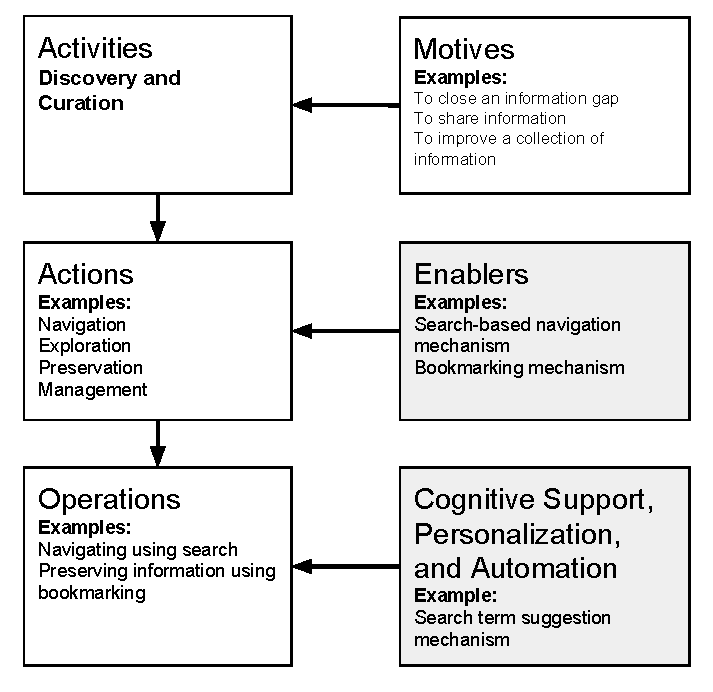
\includegraphics[width=\columnwidth]{figures/framework_overview.pdf}
	\caption{Framework Composition. The framework consists of Motives that drive Activities of discovery and curation, Actions that users undertake in order to carry on those Activities, and Enablers that the system must provision in order to support those Actions. Furthermore, Cognitive Support mechanisms enhance Enablers and make them more usable by simplifying Operations which people perform on those Enablers.}
	\label{fig:framework_overview} 
\end{figure}


{\subsection{Motives Behind Information Discovery and Curation}


There are a wide variety of user motives behind information discovery and curation, and certain aspects of these motives can significantly impact the design of an application. Understanding a user's motives can help form a conceptual model of a needed Web application and its features. The following generalizations of motives and their properties can help define conceptual models and identify primary information discovery and curation use cases.  

{\subsubsection{Motive: Closing a Knowledge Gap}
The primary motive for information discovery is usually to close a knowledge gap that occurs when the user tries to accomplish a task but lacks information to do so. 
% CUTCANDIDATE
%This motive can be of various type depending on the nature of the information need and other aspects of the given motive.        
% CUTCANDIDATE
Depending on the context in which the motive arose, an information need can have various degrees of specificity. For example, if the motive is to find inspiration for a project, the information need is vaguely defined. However, if the motive is to find a phone number of a specific business, an information need is well-defined. In some cases, the information need may be hidden and the user might not be aware of the existing knowledge gap. The specificity of an information need determines important properties of information discovery mechanisms, such as whether users can benefit more from mechanisms that allow them to specify an information need, help form an information need, or allow them to randomly retrieve information. This property has to be taken into consideration when evaluating or designing a Web application. 

The nature of an information need predetermines whether discovery is 
% respectively 
serendipitous or oriented towards fact finding. Thus, 
% depending on the user needs, 
an application can be designed to increase serendipity and opportunistic discovery or to improve purposeful fact finding. On the one hand, displaying featured content can improve serendipitous discovery because of its unexpected nature and novelty. On the other hand, using context (e.g., location and date) to tailor search results can improve fact finding. 

Another motive type for information discovery relates to the two qualities of the Web defined by Lindley et al.\cite{lindley2012s}: \textit{persistence} refers to the quality of the Web that allows people to habitually revisit Web pages and continue ongoing Web projects; and \textit{temporality} refers to the quality of the Web that allows the content of Websites to be continuously updated to provide users with new information. Persistence alone usually facilitates information \textit{rediscovery}, which is an act of refinding previously found information. However, if persistence is combined with temporality, they can facilitate discovery of new information within the same application or channel. We refer to this type of discovery as \textit{channel-based discovery}. Some of the common motives for channel-based discovery include orienting (or monitoring for updates) and opportunistic information discovery~\cite{lindley2012s}.          

The motive behind information rediscovery involves finding previously discovered information and reclosing the previously closed knowledge gap (e.g., in case the information was forgotten). It usually results in the user looking for previously found resources and Web pages. In fact, Web page revisitation is one of the most commonly performed Web browsing activities~\cite{adar2008large,cockburn2003improving}. The percentage of revisited Web pages involved in Web browsing can range from 58\%~\cite{tauscher1997people} to 81\%~\cite{cockburn2001web}. 
%Some of the reasons for revisiting pages include shopping, communication, entertainment, education, activity planning, and hobby-related information retrieval~\cite{adar2008large}.
% CUTCANDIDATE
% (e.g., travel, fitness, and cooking). 
% CUTCANDIDATE
Some Web pages and resources can be rediscovered using navigation, while others need to be previously preserved (bookmarked) to afford rediscovery. Rediscovery is one of the many ways in which information discovery and curation interweave. 
}

{\subsubsection{Motive: Supporting Future Use and Reaccess}
The main motive behind information curation is to make it possible to retrieve and use information. In order to facilitate easy information retrieval, many Web applications employ various forms of bookmarking systems. Traditionally, bookmarks must be manually organized into folders, but this method of organization is considered inefficient because folders with bookmarks become easily cluttered~\cite{abrams1998information}. Therefore, in order to efficiently support information rediscovery, Web tools need to provide mechanisms for information preservation along with information management.
}

{\subsubsection{Motive: Improving Collections}
People gather information to improve existing collections~\cite{lindley2012s}. Although some deeper motives may include self reflection or the possibility of future use, collecting information is a motive in itself. Information gathering may be stretched over a period of time~\cite{kellar2006goal}, resulting in repeated page visitation. Although information gathering comprises only 13.4\% of Web usage, it contributes to many goal-supporting activities, such as decision making and planning~\cite{kellar2006goal}.

}

{\subsubsection{Motive: Facilitating Communication}
As part of his information behavior model, Wilson identified communication of information as an outcome of information seeking. Communication can also be thought of as a motive for information discovery and curation. To support communication of information, Web tools provide mechanisms that allow various users to share information among themselves. 
%
\textit{Social bookmarking} is one popular way to preserve and share information across communities and to communicate with other users~\cite{estelles2010social}. One of the first visions of social bookmarking was associated with Web blogging. Oravec~\cite{oravec2002bookmarking} suggests that Web blogs help users annotate or bookmark important information and build a ``map'' of the Internet. The evolution of social bookmarking has led to advanced techniques for collaborative information discovery and curation. 
}

% CUTCANDIDATE
%{\subsubsection{Summary}
% CUTCANDIDATE
In summary, while it is not feasible to list all of the possible motives for information discovery and curation, this section outlined some of the key motives that can aid in developing use cases and formalizing conceptual models for Web applications. These motives also make it easier to showcase how mechanisms for discovery and curation activities (presented in the next section) complement each other.
} 
}

{\subsection{Discovery and Curation Activities}

The next part of the framework deals with the actions associated with enablers of information discovery and curation. A more detailed overview is depicted in Figure~\ref{fig:enablers}; the two main activities (discovery and curation) are decomposed into actions, and each of the actions is supported by a group of enablers (features or mechanisms) that provide means for a given action of discovery or curation in a Web application.


\begin{figure}[htp!]
	\noindent
	\centering
    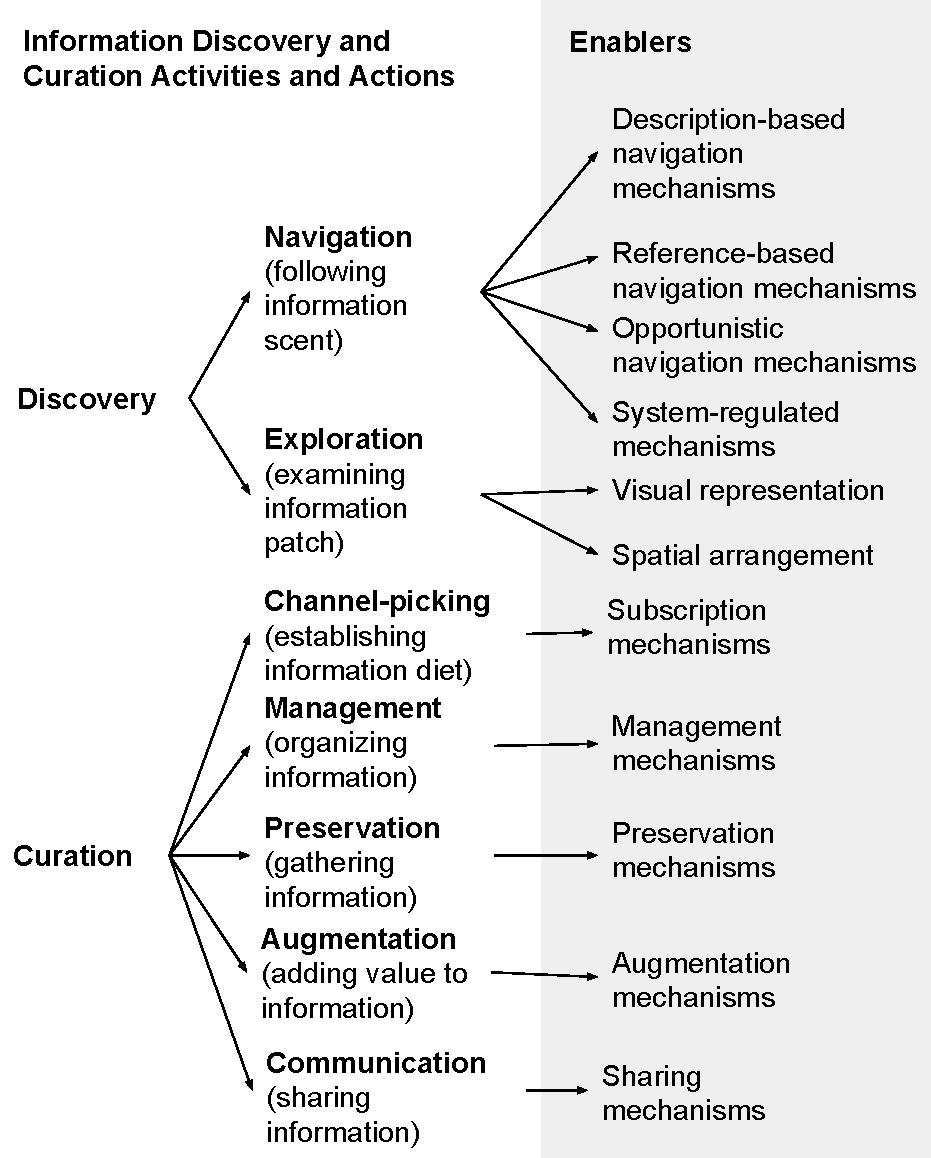
\includegraphics[width=\linewidth]{figures/framework_enablers.pdf}
	\caption{Information Discovery and Curation Activities, Actions, and Corresponding Enablers}
	\label{fig:enablers} 
\end{figure}

{\subsubsection{Action: Navigation in Discovery (Following Information Scent)}
To discover information, a user needs a way to navigate to it. Navigation action in information discovery can be thought of as following an information scent. In general, the information scent models deal with how users identify value, cost, or the access path of information sources based on proximal cues, such as links, icons, categories, etc.~\cite{pirolli1999information}. Common types of navigation actions that facilitate information discovery activity include descriptional, referential, opportunistic, and system-regulated navigation.  We describe these types of navigation actions below and direct the reader to Table~\ref{table:framework_navigation} to see an overview of these actions and the enablers possible for each action. 


\begin{table}[!htbp]
\small
\begin{tabular}{|p{0.25\linewidth}| p{0.35\linewidth}| p{0.35\linewidth}|}
\hline
\multirow{2}{\linewidth}{\textbf{Types of navigation features}} & \multicolumn{2}{ p{0.7\linewidth} |}{\textbf{Questions to be posed during the design or evaluation of  discovery and curation tools and sample features}} \\\cline{2-3}

 & Enabling mechanisms & Cognitive support, personalization, and automation \\
\hline
\textbf{Descriptional} 			& \textbf{How does the application support descriptional navigation?} & \textbf{How can descriptional navigation mechanisms be enhanced?}\\
&  Search-based navigation / Integrated search & Personalized results / Guided search\\
				
\textbf{Referential}       		& \textbf{How does the application support referential navigation?} & \textbf{How can referential navigation mechanisms be enhanced?}\\
& Categories / Facets / Filters / Tags / Search by item or resource / Integrated reference & Suggesting categories / Suggesting topics of interest / Suggesting tags / Suggesting similar resources \\
				    		
\textbf{Opportunistic}          & \textbf{How does the application support opportunistic navigation?}& \textbf{How can opportunistic navigation mechanisms be enhanced?}\\
& Opportunistic navigation feature / Integrated opportunistic navigation & Personalized opportunistic navigation \\
\textbf{System-regulated}       &\textbf{How does the application support system-regulated navigation?} & \textbf{How can system-regulated navigation mechanisms be enhanced?}\\
& Static direct display / Integrated static display / Featured content / Integrated featured content / News feed / Integrated news feed & Personalized featured content / User activity update notification / Application activity update notification / Artifact update notification \\
    
\hline
\end{tabular}
\caption{Types of Navigation Features and Related Questions}
\label{table:framework_navigation} 
\end{table}

\textbf{Descriptional Navigation (Type of Navigation Action):} A navigation action is descriptional when the user has a means of describing their information need. It is usually implemented as \feature{search-based navigation} since it allows users to enter a search query and describe what they want to find.  
% CUTCANDIDATE we mention Stumbleupon below and integration
%Some applications use other methods of navigation, such as StumbleUpon and some Web applications are \feature{integrated} with others, enabling users to search multiple Websites at once. 
% CUTCANDIDATE 
Some modern descriptional navigation systems are voice-activated.  
%
% CUTCANDIDATE
%There are numerous ways in which descriptional navigation supports information discovery. Search-based navigation often serves as an entry point for information seeking~\cite{levene2011introduction}. When the motive behind information discovery has a well-articulated information need, then the user can express their information need by entering a search query. 
% CUTCANDIDATE

Descriptional navigation enablers can also help to rediscover information, but it is not always a reliable way of rediscovery ~\cite{cockburn2003improving}. In information portals that provide access to fairly ambiguous information and that have regularly updated information flow, the search-based navigation enablers are usually designed around retrieving information related to some general topic. In order to make search-based navigation a reliable way to rediscover information, it must return consistent results. 
} % end subsection


\textbf{Referential Navigation (Type of Navigation Action):}
A navigation action is referential when the user finds a reference to the term that they are looking for, such as a link or icon. This reference represents an information scent. The underlying assumption of this type of navigation action is that the user can recognize the needed information or a reference to it as they see it~\cite{waterworth1991model}. 

Referential navigation enablers can take many forms. Some common types are \feature{categories}, \feature{facets}, \feature{filters} and \feature{tags}. In some applications, users can search by a given \feature{resource}. For example, YouTube provides a playlist with music related to the currently playing song. Information scent representatives may also reference sources outside of the given system, enabling another type of \feature{integration} of Web applications. 
%
Referential navigation enablers can help the user identify their information needs by suggesting terms, topics or categories to use, and therefore, direct the user to relevant resources~\cite{levene2011introduction}. It can also help narrow the results to a specific type of resource so that further discovery is bounded by that type. For example, TripAdvisor helps narrow search results by allowing users to choose among hotels, flights, vacation rentals, restaurants and destinations.

\textbf{Opportunistic Navigation (Type of Navigation Action):}
Opportunistic navigation is a type of navigation action where the user `randomly' navigates through resources and Web pages. We call this `opportunistic' because it is not truly random, but its serendipitous nature makes users feel like it is. This type of navigation action is especially useful when the information need is fully undefined.
%
Many applications support opportunistic jumping from one resource to another. For example, StumbleUpon makes it possible to explore the Web in general---other Websites and Web applications, allows for \feature{integrated} opportunistic navigation---whereas Wikipedia provides opportunistic access to its own articles. 


\textbf{System-regulated Navigation (Type of Navigation Action):}
Web applications often display information without the user's active participation. This information can be a \feature{news feed}, \feature{featured} deals or articles or other types of content. We refer to this type of navigation action as system-regulated because it occurs when the application brings the content to the user instead of the user applying any effort to find content. It differs from opportunistic navigation because the the user cannot choose when to observe new information; instead, all updates are regulated by the application. 
%
One application that supports system-regulated navigation action is Yelp. As soon as the user enters the site, this tool displays featured restaurants as well as the user's recent activities. As with any other navigation actions, system-regulated navigation can ensure cross-application \feature{integration} by displaying content from other Web applications. 


{\subsubsection{Action: Exploration in Discovery (Examining Information Patches)}
Exploration of resources is another action that facilitates the activity of information discovery. Visual and spatial cues, which help representing single or multiple resources, serve as enablers for this action by allowing users to conveniently examine information patches (please refer to Table~\ref{table:framework_exploration}). 

\begin{table}[!htbp]
\small
\begin{tabular}{|p{0.25\linewidth}| p{0.35\linewidth}| p{0.35\linewidth}|}
\hline
\multirow{2}{\linewidth}{\textbf{Types of exploration features}}   & \multicolumn{2}{ p{0.7\linewidth} |}{\textbf{Questions to be posed during the design or evaluation of  discovery and curation tools and sample features}} \\\cline{2-3}

 & Enabling mechanisms & Cognitive support, personalization, and automation \\
\hline
\textbf{Visual and textual cues of multiple resources} & \textbf{How does the application use visual and textual cues to help identify resources of value?} & \textbf{How can visual and textual cues of multiple resources be enhanced?}\\
& Visual preview / Textual preview & Personalized visual preview / Personalized textual preview \\
\textbf{Visual and textual cues of a single resource} & \textbf{How does the application use visual and textual cues to help identify the value of information within a resource?} & \textbf{How can visual and textual cues of a single resource be enhanced?}\\
& Visual cues / Textual cues & Personalized visual cues / Personalized textual cues \\                
\textbf{Spatial proximal cues of multiple resources} & \textbf{How does the application use spatial proximal cues to effectively present multiple resources?} & \textbf{How can the use of spatial proximal cues be enhanced to effectively present multiple resources?}\\
& List / Grid / Gallery / Spatial semantic / Consistency & Personalized arrangement of multiple resources\\
\textbf{Spatial proximal cues of a single resource} & \textbf{How does the application use spatial proximal cues to effectively present information within a single resource?} & \textbf{How can the use of spatial proximal cues be enhanced to effectively present information within a resources?}\\
& Spatial semantic / Consistency & Personalized arrangement of information within a resource  \\ 
     
\hline
\end{tabular}
\caption{Types of Exploration Features and Related Questions}
\label{table:framework_exploration} 
\end{table}

\textbf{Visual and textual previews (exploration enablers):} Abrams et al.~\cite{abrams1998information} identified link representation as one of the problems with traditional bookmarking. Analogous with browsing through a bookmark manager, identifying relevant information when browsing through links in a Web application can be a challenging task. \feature{Visual previews} and \feature{textual previews} make it easier to evaluate the relevance of resources by providing the user with more information scent and thereby serving as enablers for the action of exploration. Many social bookmarking systems, such as Scoop.it! and Pinterest, support visual previews of bookmarked pages. Delicious is a social bookmarking application that lacks this type of link representation support, and so it is harder to determine if a link will lead to a relevant resource.

\textbf{Visual and textual cues (exploration enablers):} \feature{Visual and textual information cues} are also important enablers for the action of exploration. Not only do they help navigation within the resource or Web page, but they can also contribute to the learning experience. For example, if the user would like to know what something looks like, they can learn it from the representation in question.  

\textbf{Spatial visualizations (exploration enablers):} Similar to link representation, effective spatial visualization of numerous links can be another challenge of supporting exploration of diverse content~\cite{abrams1998information}. Therefore, a semantic to the \feature{spatial arrangement} of information (single and multiple resources) is of major importance. Information discovery applications often employ sophisticated ways of spatially arranging resources to make it easier to browse through large amounts of information. Common ways of arranging multiple resources include \feature{list}, \feature{grid}, and \feature{gallery} layouts. Additionally, \feature{consistency} in the way multiple and single resources are represented is another enabler that helps form a conceptual model of how the application can be used and provides some degree of predictability~\cite{norman2002design}.
} % end section

{\subsection{Activity: Curation}
Information curation is a common activity across many information discovery applications. By asking questions about application design with regards to information curation designers can find ways to add value to information and enable information discovery over time. 
%
Information discovery applications vary from being completely socially curated and populated by users, to those that lack any curation mechanisms. 
By definition, digital information curation is the notion of managing, preserving, and adding value to collections of information ~\cite{beagrie2008digital,whittaker2011personal}. Thus, curation activity consists of actions such as information management, preservation, information augmentation, sharing, and channel-picking. Refer to Table~\ref{table:framework_curation} for this part of the framework.

\begin{table}[!htbp]
\small
\begin{tabular}{|p{0.2\linewidth}| p{0.45\linewidth}| p{0.4\linewidth}|}
\hline
\multirow{2}{\linewidth}{\textbf{Types of curation features}}   & \multicolumn{2}{ p{0.8\linewidth} |}{\textbf{Questions to be posed during the design or evaluation of  discovery and curation tools and sample features}} \\\cline{2-3}

 & Enabling mechanisms & Cognitive support, personalization, and automation \\
\hline
\textbf{Management} & \textbf{How does the application support management of information?} & \textbf{How can management of information be enhanced?}\\
& Public or private collection-based categorization / Public or private tag-based categorization & Suggesting collections / Suggesting tags / Automated classification into collections / Automated tagging \\
\textbf{Preservation} & \textbf{How does the application support preservation of information?} & \textbf{How can preservation of information be enhanced?}\\
& Internal preservation of internal resources / Internal preservation of external resources / External preservation of internal resources & History / Suggested preservation  \\
\textbf{Augmentation} & \textbf{How does the application support augmentation of information?} & \textbf{How can augmentation of information be enhanced?}\\
& Annotation / Evaluation & Automated augmentation / Suggested augmentation \\ 
\textbf{Sharing} & \textbf{How does the application support sharing of information?} & \textbf{How can sharing of information be enhanced?}\\
& Adding resources / Internal sharing / External sharing & Automated sharing / Suggested sharing \\
\textbf{Channel-picking}  	& \textbf{How does the application support the user in establishing their information preferences?} & \textbf{How can establishment of information preferences be enhanced?}\\
& User subscription / Site subscription / Artifact subscription & Suggesting users for subscription / Suggesting artifacts for subscription / Automated subscription \\     
\hline
\end{tabular}
\caption{Types of Curation Features and Related Questions}
\label{table:framework_curation} 
\end{table}

% Elena being consistent with formatting above ...
\textbf{Action: Information management.} Information management is one of the key actions of the information curation activity ~\cite{beagrie2008digital,whittaker2011personal}. Its enablers are prevalent in applications that have a lot of information that is hard to categorize automatically or can mean something different for each user. In the context of Web information management, \feature{tag} and \feature{collection-based} information categorization enablers play major roles.
%
Resource categorization also helps establish relationships between various resources ~\cite{beagrie2008digital,whittaker2011personal}. Tagging can aid rediscovery and discovery in a socially curated space, as well as add more value to resources~\cite{gruber2007ontology}. Sample applications that facilitate these types of information management actions are Pinterest, a tool that supports tagging and collection-based categorization, and Tumblr, a tool that supports tagging.
%} % end subsubsection

\textbf{Action: Information preservation.} Information preservation is a common information curation action that is usually performed with the intent of revisiting information~\cite{abrams1998information,whittaker2011personal}. However, information gathering that involves information preservation is sometimes performed with just the goal of collecting information~\cite{lindley2012s}. 
%
Bookmarking is a traditional type of information preservation action. Having the \feature{internal preservation of internal resources} enabler means bookmarking resources can be reaccessed within the same application. Such an enabler facilitates information curation within the system. The \feature{internal preservation of external resources} enabler facilitates bookmarking other Web pages within an application. Having the \feature{external preservation} enabler means bookmarking resources so that they are available through other bookmarking systems. An application must facilitate integration with other applications to enable the external preservation type of information preservation action~\cite{abrams1998information}.
%
% CUTCANDIDATE
%For example, in the We Heart It image discovery application users can preserve \feature{internal  information} using \feature{internal collections} and they can add information from \feature{external} websites. However, there are no integrated means for bookmarking \feature{internal content} using other bookmarking systems. 
% CUTCANDIDATE 
%} % end subsubsection

\textbf{Action: Augmentation.}
One of the most important actions of the digital curation activity is augmentation: adding value to information ~\cite{beagrie2008digital,whittaker2011personal}. It is often performed within social bookmarking systems, and many Web applications allow users to add value to the resources they curate. 
%
One way to augment information is by \feature{annotating} it with comments and descriptions. Annotations are metadata, such as comments and reviews, attached to a resource that makes it easier to search for and interpret information. For example, Yelp and TripAdvisor largely rely on reviews written by their users. 
%
\feature{Evaluation} enablers can have various forms. They usually take place in socially curated information systems. However, evaluation can also contribute to personal reflection and information preservation. Many applications allow users to perform the evaluation type of augmentation action by providing some means for rating of resources or recording other forms of approval or disapproval, such as ``I like this" and ``I dislike this" buttons on YouTube.
%} % end subsubsection

\textbf{Action: Sharing.}
The action of information sharing is key to empowering social information curation ~\cite{beagrie2008digital}. Therefore, the main enablers that facilitate the action of sharing are the adding of resources, and external and internal information sharing mechanisms.
%
\feature{Adding resources} not only facilitates global Web information curation, but it also scales the information available through the system, providing more opportunities for information discovery. Resources can be created by users themselves, taken from some other sources online, or both. For example, YouTube allows users to upload their own videos, whereas Pinterest permits adding images from other sites in addition to users' personal images. 
%
Sharing resources through different media and resharing them within the Web application facilitates channel-based information discovery within the media channels. Information discovery applications commonly allow for sharing information on popular networking sites outside the application.
%} % end subsubsection


\textbf{Action: Channel-picking}. Channel-picking is an action of selecting information sources. A common enabler for this action is subscriptions that help users follow the news~\cite{java2007feeds}. To support channel-based type of discovery, an application must provide a subscription enabler. For example, Rotten Tomatoes allows \feature{subscriptions} to \feature{newsletters}, but it does not allow subscriptions to movie critics that would be allowed with a user-based subscription enabler such as the one in Pinterest. 
%
In some applications, the content is updated and curated by users, and users can \feature{subscribe} to other \feature{users} or \feature{artifacts}. Similar to site subscriptions, user and artifact subscriptions are subscriptions to activity updates. These subscription mechanisms help with networking and provide awareness about other users' activities~\cite{millen2005social}. Such subscriptions also help filter new content delivered to the user. 
%} % end subsubsection
} % end subsection

% CUTCANDIDATE
%{\subsection{Summary}
% CUTCANDIDATE
In summary, information discovery and curation tools can have different implementations depending on the motives behind the activities. The enablers presented in this section can help facilitate different actions associated with information discovery and curation activities. However, the activities can be significantly improved by additional support and automation, as described in the next section.

%} % end section

{\subsection{Cognitive Support: Enhancing the Discovery and Curation Experience}

The information discovery and curation enablers just presented are design elements that afford various operations. For example, the search feature enables typing in a query and searching for information. These operations can be further supported by another set of design elements that introduce cognitive support for those operations. Cognitive support elements are elements that make user experience smoother even if a given operation could be performed without it. They often become enhancements on existing enablers allowing for less cognitively demanding operations. The primary goal of this part of the framework (see right column of Table 2) is to highlight opportunities for improvement over various information discovery and curation enablers.
%

Strategies for improvement include providing additional cognitive support for a given operation, personalizing the user experience, and automating an operation. Not all of the strategies are feasible for every single operation, and some operations can be supported in multiple ways. The following  outline some of the possibilities for advancing information discovery and curation features. 

{\textbf{Cognitive Support: Enhancing Navigation.}
There are two common methods of enhancing information discovery when search-based navigation is used (see Table~\ref{table:framework_navigation}). The first method entails returning personalized results when the user enters a search query. \feature{Personalization} can be accomplished using a variety of techniques, including predefined user preferences, social interactions, context, browsing history, etc. The second method is to \feature{suggest search terms} to make it easier for the user to formulate their information need. For example, Yelp suggests search terms as the user enters their query.

To further support referential navigation, applications can \feature{personalize} reference suggestions, such as \feature{categories}, \feature{tags}, and \feature{topics} of interest. They can also suggest relevant resources based on the one that the user already selected. As an example, after a user clicks a `pin', Pinterest showcases other similar `pins'.

For opportunistic navigation, Web tools sometimes allow users to \feature{personalize} types or categories of information that they the users would like to discover. StumbleUpon allows users to not only choose topics of interests, but it can also help them discover new promising topics.


Featured content can also be \feature{personalized} to improve information discovery with system-regulated navigation. For example, Yelp showcases restaurants from a predefined area, such as the city where the user is from.

Finally, to make better use of subscribed content and to reduce human efforts when searching, an application can support various \feature{notification mechanisms}. These can advise the user about updates on the \feature{Website content}, various \feature{artifacts}, and activities of other \feature{users}.  

} % end subsection
{\textbf{Cognitive Support: Enhancing Exploration.}
\feature{Personalization} of the \feature{spatial} information representation usually has limited support in Web applications. Presumably, it is because consistency is more welcomed within information discovery applications than spatial personalization. However, it is still possible to personalize the arrangement of multiple resources or information within a single resource. 
%
\feature{Visual} and \feature{textual personalizations} are more common, especially when the content within the application is curated by its users.  For example, Flickr Web application for managing and sharing photographs personalizes album covers so that they are easier to rediscover. 
% Similarly, `pinboards' on Pinterest have personalized cover images.


{\textbf{Cognitive Support: Enhancing Curation.}
Information management can be improved if the system helps the user make decisions about information categorization or tagging (see Table~\ref{table:framework_curation}). Alternatively, information can be \feature{categorized} or \feature{tagged automatically}. For example, when the user bookmarks a restaurant on Yelp, it is automatically categorized. The user can filter bookmarks by category whenever they go into the embedded bookmark manager. 

Preservation operations can also be automated. An example of the most common automatic preservation mechanism is \feature{history}. Applications such as YouTube and Google Maps preserve users' browsing history so that they can review it later. Additionally, preservation mechanisms can be \feature{suggested} to the user.
% 
YouTube allows users to \feature{automatically share} information about their activities, such as comments,  added videos, liked or disliked videos, and created playlists. In general, socially curated spaces offer \feature{sharing channels} to support convenient information communication.
%
Augmentation is another aspect of information curation that can be either \feature{automated} for or \feature{suggested} to the user. For example, Yelp asks users to rate the places which the application identifies as having been visited by the user. 

Notification mechanisms enable user awareness about new content on the subscribed channel~\cite{millen2005social}. Web applications that facilitate rapidly updating content support various notification mechanisms, such as messages within the application, informative emails, and smartphone notifications. Many types of notifications include suggested users or artifacts to follow. Some Web tools automatically subscribe users to notifications, usually during the registration process.
} % end subsection

% {\subsection{Summary}
In summary, providing cognitive support, personalization, and automation dramatically improves the user experience when people interact with information discovery and curation systems. The framework can be used for identifying gaps in information discovery support and developing new technologies as described in the following section.  
}

\section{Framework Validation}
\label{section:validation}
In order to validate the conceptual framework and verify its stability, we used it to design a tool for location based photograph discovery and curation, we used it to evaluate five of the applications that were used in the construction of the preliminary framework: Pinterest, Google Maps, Wikipedia, Delicious, and Yelp. Due to space limitations, we only present the evaluation for one of the tools, Pinterest. The other tool evaluations and the location based discovery tool description can be found in~\cite{voyloshnikova2015}. As for Pinterest, we first summarize our observations resulting from asking the questions from the framework in a systematic manner. Based on our assumptions, judgment, and use of the framework, we propose directions for future development and reflect on certain needed mechanisms, as not all mechanisms are always required. 

Pinterest is a Web application designed for image discovery and curation, oriented towards finding inspiration and collecting knowledge about hobbies and interests~\cite{gilbert2013need,zarro2012pinterest,ottoni2013ladies}.  Users of Pinterest are commonly referred to as `pinners'. Resources on Pinterest are called `pins', and each `pin' consists of an image, a short description, the user's name, and the name of the collection that the pin belongs to. More information is available once the user clicks on a `pin'.

Motivated by the desire to gain inspiration and knowledge, Pinterest users have either under-defined or absent information needs. Other motives for using Pinterest could be to rediscover previously found information (and possibly use it), to be oriented about new `pins' that emerge from subscribed channels, and to gather information for future rediscovery and the act of collection itself.

Navigation in Pinterest is mostly supported by descriptional, referential, or system-regulated mechanisms. Although an explicit \feature{opportunistic navigation mechanism} is absent, both descriptional and referential mechanisms usually return novel and serendipitous results to facilitate opportunistic browsing. Descriptional navigation is enabled with a \feature{guided search} mechanism that suggests search terms to the user. 

Referential navigation is enabled in Pinterest using a range of techniques. To support articulation of an information need, a \feature{category-based} navigation mechanism makes suggestions on subcategories or interests. Through clicking on a `pin', the user can see related resources, enabling \feature{resource-based} referential navigation. Most of the images on Pinterest are `pinned' from other Websites, and users are provided with links to their original sources. Therefore, Pinterest supports \feature{integrated} referential navigation.

System-regulated navigation within Pinterest is highly personalized. When the user enters the site, they see a history of their own information gathering activities and updates from the people they are subscribed to. Additionally, the application suggests \feature{featured} `pins' based on the user's interests.

To reinforce the discovery of visual data, Pinterest provides extensive support for various exploration mechanisms. Multiple resources are represented in a \feature{gallery layout}, often referred to as a 'pinboard'. This layout provides good spatial support for exploration and makes it easier to build a mental model of the tool by drawing analogies with a real pinboard. Users can create multiple `pinboards' (also known as `boards') which have \feature{personalized} covers to enhance future exploration and rediscovery.
%
A single resource does not have a lot of distinct spatial arrangements, however, it provides a visual glimpse into what can be found on the Website that the image came from, with \feature{textual preview} being limited to the address of the Website. 

Information management is accomplished through sorting `pins' into different collections (`pinboards') thus enabling \feature{collection-based classification} and \feature{internal preservation of internal and external resources}. All user information collecting actions are \feature{automatically} preserved and displayed. Users can augment the information pool by uploading new `pins', commenting on existing `pins', or adding descriptions. Users can also \feature{internally share} 'pins' among themselves. Channel-picking actions are carried out by following or \feature{subscribing} to users or individual `pinboards'. The system also \feature{automatically} sends \feature{notifications} though emails and \feature{suggests} new `boards' to follow.

Applying the framework to Pinterest revealed that it employs a  variety of techniques to facilitate information discovery and curation. However, individual mechanisms could be further improved. For example, \feature{textual previews} of multiple and individual resources is rather limited and provides little insight into what information source Websites actually contain. Furthermore, Pinterest could benefit from \feature{automatically classifying} `pins' into `boards' because finding an appropriate `board' for a `pin' can be difficult when a user has a large number of existing `boards'. Overall, Pinterest provides rich support for information discovery and curation, and in some ways, enables each of the discovery or curation actions of the conceptual framework. 
} % end section

\section{Research and Design Implications}
\label{section:implications}
The conceptual framework for information discovery and curation is designed to perform formative and summative evaluation of existing Web applications and to reveal how these tools support information-related activities in question. The framework as a tool and its ability to guide the process of analyzing Web applications makes it broadly applicable in research and Web design. 

In the previous section, we demonstrated how the framework can be used to reveal missing features in tools. Using similar methods, the framework can also be applied to compare different Web applications. When used for evaluation, the framework helps to identify which areas of a tool require further attention. Therefore, the framework can be helpful for designers who wish to improve existing tools or get ideas for new information discovery and curation applications. 

Factors and questions of the framework are there to guide the developer and may expose gaps, but they do not dictate which features should be in an application. It is up to designers to decide whether to close those gaps and some gaps cannot be closed because of certain constraints or trade-offs that have to be made, such as data type and system design.

% CUTCANDIDATE
%User interface designers face certain trade-offs when developing applications. Therefore, it is not always advantageous to implement all missing features. For example, providing the support to customize spatial arrangement of multiple resources can undermine the consistency of their representation. 
% CUTCANDIDATE

Even though applying the framework requires initial expertise and critical reasoning, it opens up opportunities for research and practice. 
For the research domain, the framework can serve as a guide for drawing distinctions between different Web-based information discovery and curation applications, finding gaps in tools, and selecting cases for studies based on required functionality. 
While, systematic evaluation of Web tools for information discovery and curation helps the designer improve user experience and gain better understanding of information behaviour within a given system. 

\section{Future Work and Conclusions}
\label{section:future_work}
In our study, we analyzed information curation and seeking tasks and developed a conceptual framework of factors and questions that are important when building and evaluating Web information discovery and curation tools. We then evaluated and iteratively refined the framework by analyzing 20 different information discovery applications and provided concrete examples of tool support addressing various concepts of the framework. Finally, we validated the framework by reevaluating five of the previously examined tools and used it to design a novel application (described in ~\cite{voyloshnikova2015}). 

The current version of the framework is designed to be generally applicable to information discovery applications. Finding ways to instantiate the framework and extend it for use in domain-specific practices could serve as a potential future research goal. For example, video discovery and curation activities have unique properties related to the type of data to be discovered---information is mostly found in the video itself, and it cannot be viewed all at the same time. Hence, the framework could be extended to address domain-specific challenges. 
%
Another potential research direction would be to expand our investigation to include factors that influence the need for one information discovery type over another and further deepen an understanding of the relationships between the motives for information discovery and curation activities and information discovery types. 
% CUT CANDIDATE
%Additionally, one could investigate how collaboration in information discovery and curation relates to the conceptual framework. Generally, collaboration mechanisms in most Web information discovery applications are limited to information sharing, public information augmentation and tagging. However, collaboration often involves other activities, such as communication, coordination, and other domain-specific shared activities.
% CUT CANDIDATE

Our framework opens up opportunities for structured information discovery and curation tool evaluation and design. As more tools are being developed within the social space of information discovery and curation, understanding how these tasks can be supported promises advancements in how Web applications are designed.

\section*{References}

\bibliography{mybibfile}

\end{document}